\documentclass[UTF8]{article}
\usepackage{graphicx}
\usepackage{hyperref}
\hypersetup{
    colorlinks=true,
    linkcolor=blue,
    filecolor=magenta,      
    urlcolor=cyan,
}
\graphicspath{ {images/} }
\begin{document}

\title{%
 \Huge \textbf{EEEE485 Tech Memo}  \\
  \begin{flushleft}
   \Large \textbf{From:} Trevor Sherrard \\
         \textbf{Partner:} Rodney Sanchez  \\
         \textbf{To:}  Dr. Ferat Sahin -- Section L2 \\
         \textbf{Course:} Robotics Systems [EEEE 485] \\
         \textbf{Date Due:} 12/16/2016 \\
		 \textbf{Subject:} Weather Detection Robot Project
		 \end{flushleft}}
\maketitle
\newpage
\large
\section{Abstract}
This project required the design of a differential drive robot with a specific characteristic. In this project the characteristic that was chosen to do weather detection. Logistic regression was implemented to classify the readings from an atmospheric sensor. Temperature, humidity and pressure were used to classify the weather a dataset of the Rochester area. Remote control was also performed using a Microsoft Xbox controller and a XBEE wireless radio. A Raspberry Pi was used to perform the actual classification of weather data, while the Teensy was used to read from sensors and control the motors accordingly.

\section{Theory}

\subsection{Multivariable Logistic Regression}
Multivariable logistic regression is a model that separates the input into 2 categories, "on" or "off". This model predicts some probability for the latter categories. Multivariable logistic regression works on similar concepts except it produces a probability for all possible classes. To do so the algorithm first sends a vector of features through a set of weights then it sends the received value through a Softmax algorithm that produces a probability of for a given class. The highest probability is then chosen and compared to the actual class. The loss is then calculated using cross entropy layer to produce an error or loss. The weights are then changed by using stochastic gradient decent. Stochastic gradient decent takes in weights and updates them by performing the gradient of the error and subtracting it from the previous weight value.

\subsection{XBEE Communication}
Wireless radio communication was implemented through the use of XBEE modules. The modules were used to transmit characters that were send through MATLAB code. The characters would then be collected by a teensy that used the given information to change the mode of the robot, read from the weather sensor, or allow joystick control of the robot. XBEE radios use the ZigBee wireless protocal which, in this case, is effectively wireless USB serial.

\subsection{$I^2C$ Protocol}
$I^2C$ communication uses 2 types of line SDA, serial data line, and SCL, serial clock line. The bus in the I2c communication serves 2 porpuposes, master that generates a clock and initiates communication with the slaves. It can also be a slave node that takes in a clock when addressed by the master. It has different type of message protocol single were the master reads from the slave. The master can also read from the slave which is denoted as single message. Then there is combined messages were the master reads or writes from or to multiple slaves.

\vspace{4mm}
\noindent
This protocol can operate at very fast clock speeds. In the case of the Sparkfun BME280 Atmospheric sensor, the data can be quicly read from the sensors on the chip over the $I^2C$ protocol. 

\subsection{Closed Loop Motor Control}
Closed loop motor control is the elementary feedback system for motor control. That is, a nominal speed is set, and the robot is allowed to move around at that set speed. The encoders on each motor use timer interrupts to get the ticks per a user set period. These ticks per period are then converted to an RPM value. Each iteration through the ardunio program's loop the nominal value is compared to the actual value from the encoders. The control loop will then write the offset to the motors to compensate for the speed error. 


\section{Results and Discussion}
\subsection{Nominal Operation}
The MATLAB script mapped values from the Xbox controller to values that the XBEE would be able to send over serially. The joystick value is normally -1 to 1 where 1 is full forward.  This value was then mapped to 0 to 600. This value was read seperatly for each joystick on the controller. each maginitude was calculated and sent over XBEE wireless serial preceded by a control character that indicated which joystick the magnitude was comming from. This allowed the robot to be remotely driven in "tank drive". This means that each wheel direction and magnitude are controlled independently with two joysticks.

\vspace{4mm}
\noindent
The robot had two main modes of operation, weather mode and demo mode. The robot defaulted into demo mode when it was powered on. This mode waited for commands to be sent to the teensy via XBEE that would allow it to be remote controlled. This mode also check for the signal from the Xbox controller that would activate the weather classification sequence. When the button was pushed, one hundred samples were taken from the weather sensor and averaged together. These averaged values (Temperature, Humidity, Pressure) were sent over serial to the Raspberry Pi preceded by a identification character for parseing. On the Recieving end, the Raspberry Pi splits this string by spaces and extracted the actual floating point value of each metric. These values were then put into the classifier which output the expected weather condition. This value was then sent back to the Teensy, where a pre-programmed motion would be executed to indicated the predicted weather.

\vspace{4mm}
\noindent
If the robot received the command to enter into demo mode, the isWeatherState bool was toggled to false. Once in demo mode, the robot would start to continously poll the Ultrasonic distance sensor and the line following sensor. The standard line following algorithm is as follows: On line $\rightarrow$ arc right, Off Line $\rightarrow$ arc left. If the distance read from the ultrasonic sensor is below a threshold, swing off the line to avoid the obstacle $\rightarrow$ rejoin the line and begin line following algorithm. For a more detailed graphical representation of the control scheme of the robot, see figure 3.1.

\begin{center}
\textbf{Figure 3.1} \\
\includegraphics[scale=.20]{flowchart}
\end{center}

\subsection{Power System}
The power system was split into two rails. The first being the $6V$ rail that powered the motor driver directly and thus the motors themselves. The other rail opperated at $5V$ supplied from a portable phone charger battery. This was put directly into the power supply of the Raspberry Pi. In turn, the Raspberry Pi powered the teensy over the USB connection. This was an important design choice because it made use of the 5V regulaters built into the USB controller for the Raspberry Pi. This ensured that the teensy would operate within the nominal ranges for the USB specification. See Figure 3.2 for a picture of this subsystem.
\begin{center}
\vspace{3mm}
\textbf{Figure 3.2}\\
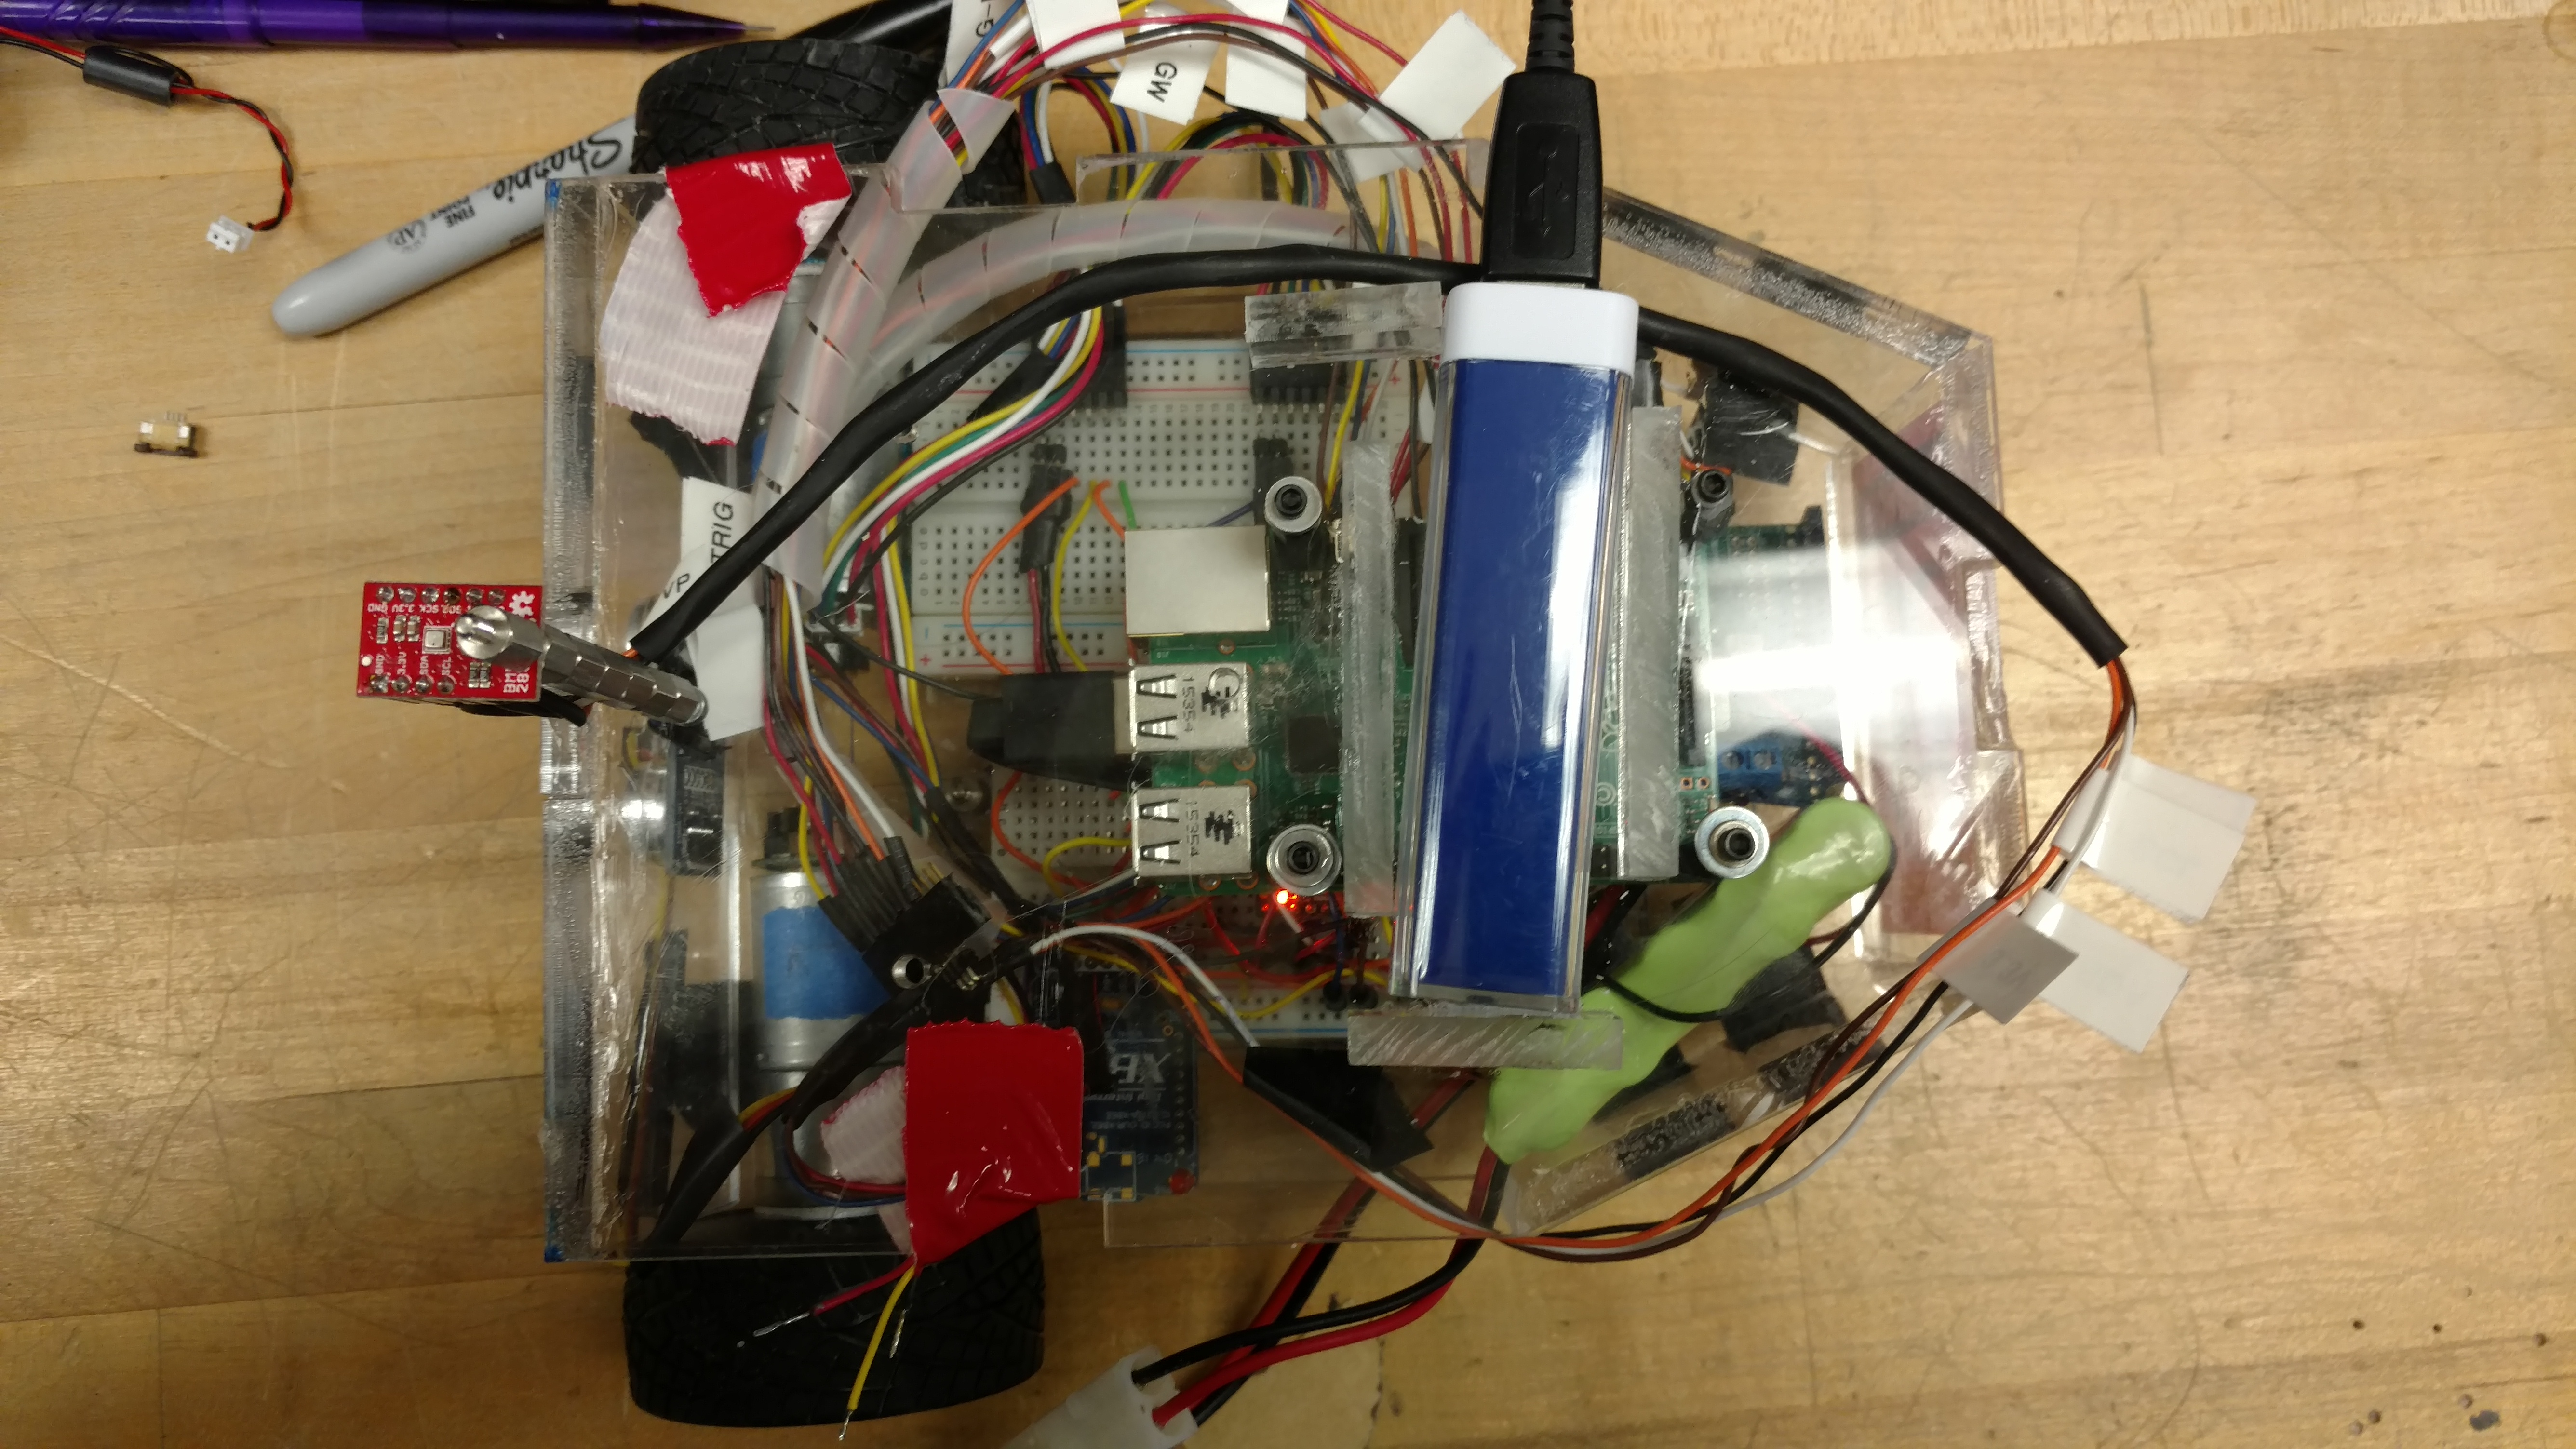
\includegraphics[scale=.05]{IMG_20161215_151223041} \\
\end{center}

\subsection{Wire Organization}
All sensor wires passed through a handmade connector that allowed for quick debugging of sensor connections. This also allowed sensors wire that needed to be different lengths to reach their respective sensors to be well organized.

\subsection{Machine Learning}
The multivariable logistic regression classifer was used a dataset of daily Rochester area weather from 2013. This data was hand scraped from \href{https://www.wunderground.com/}{wunderground.com}. The classifier was tested on seperate labeled points pulled from the same website from 2015. The accuracy of the classifer is shown in the confusion matrix in figure 3.4. This is obtained from running the classifer over the known labeled data and then checking the predicted label with the actual label.

\begin{center}
\textbf{Figure 3.4} \\
\includegraphics[scale=1]{ConfusionMatrix}
\end{center}

\subsection{Mechanical Design}
The robot's physical design had a few modifications from the design to execution phase. Originally the robot was design to be weather proof. The robot was originally designed enclosed on all sides with a physical dome mounted on top for the Sparkfun BME 280. Constraints on the size of plate for the acrylic led the robot to be modified to a more open design to accommodate for both the Teensy and the Raspberry Pi. The sides were the stripped and the mates for the front plate were then made which led to error in the fitting of the plate. The overall design was low to the ground to accommodate for the line sensor which has an effective range 3 mm. See figure 3.5 for a picture of the physical chassis. 
\vspace{6mm}
\begin{center}
\textbf{Figure 3.5} \\
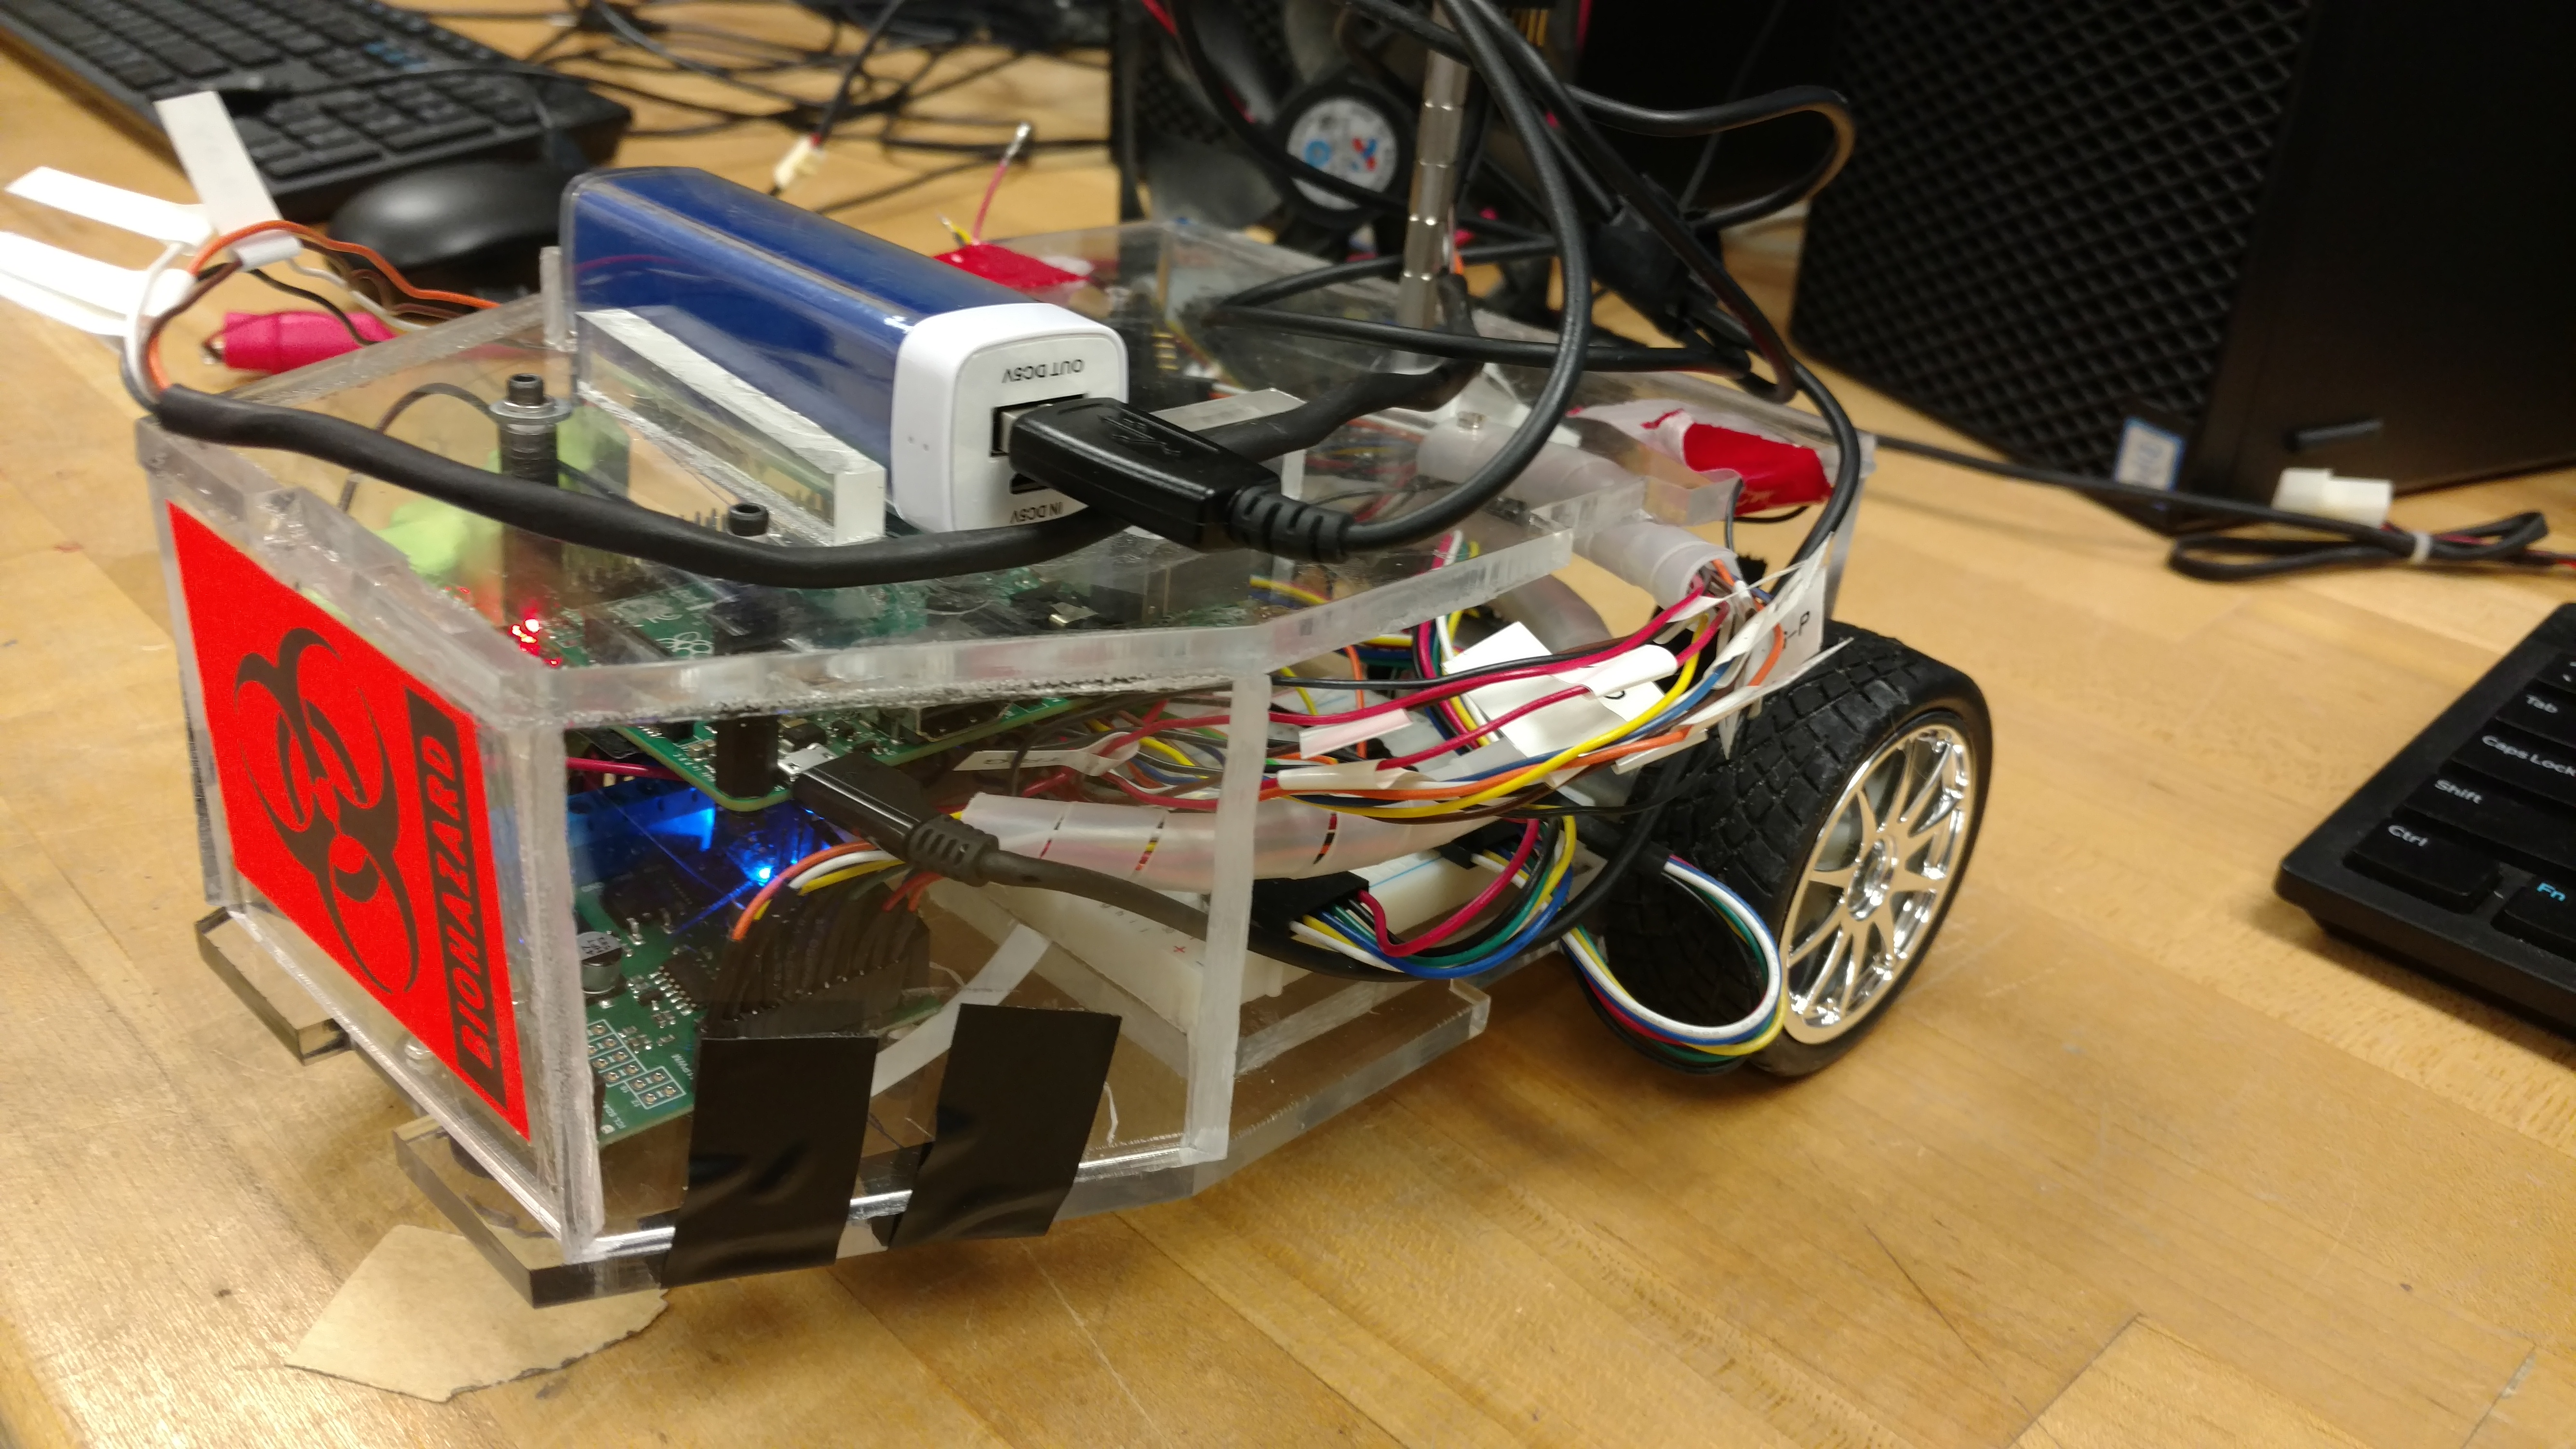
\includegraphics[scale=.06]{Chassis}
\end{center}

\section{Conclusion}
Overall, the robot worked as outlined in the original project proposal. The robot was able to sucessfully follow dark lines on the floor. The robot was also able to stray off the line if an object was detected during line following sequence. It could reliably resume the line following algorithm after the obstacle was avoided. 

\vspace{4mm}
\noindent
The remote control mode also worked reliably. The robot was able to take an average weather value from the sensor and accurately classify the weather condition. The only issue that the classifer had was that there was an abundant amount of "cloudy" days. This being the case, there are some false classifications of points as "cloudy". This would be easily fixed if more data was given to the classifer from another year. 

\end{document}

